
\documentclass[letterpaper, 12pt]{book}\usepackage[]{graphicx}\usepackage[]{color}
%% maxwidth is the original width if it is less than linewidth
%% otherwise use linewidth (to make sure the graphics do not exceed the margin)
\makeatletter
\def\maxwidth{ %
  \ifdim\Gin@nat@width>\linewidth
    \linewidth
  \else
    \Gin@nat@width
  \fi
}
\makeatother

\definecolor{fgcolor}{rgb}{0.345, 0.345, 0.345}
\newcommand{\hlnum}[1]{\textcolor[rgb]{0.686,0.059,0.569}{#1}}%
\newcommand{\hlstr}[1]{\textcolor[rgb]{0.192,0.494,0.8}{#1}}%
\newcommand{\hlcom}[1]{\textcolor[rgb]{0.678,0.584,0.686}{\textit{#1}}}%
\newcommand{\hlopt}[1]{\textcolor[rgb]{0,0,0}{#1}}%
\newcommand{\hlstd}[1]{\textcolor[rgb]{0.345,0.345,0.345}{#1}}%
\newcommand{\hlkwa}[1]{\textcolor[rgb]{0.161,0.373,0.58}{\textbf{#1}}}%
\newcommand{\hlkwb}[1]{\textcolor[rgb]{0.69,0.353,0.396}{#1}}%
\newcommand{\hlkwc}[1]{\textcolor[rgb]{0.333,0.667,0.333}{#1}}%
\newcommand{\hlkwd}[1]{\textcolor[rgb]{0.737,0.353,0.396}{\textbf{#1}}}%
\let\hlipl\hlkwb

\usepackage{framed}
\makeatletter
\newenvironment{kframe}{%
 \def\at@end@of@kframe{}%
 \ifinner\ifhmode%
  \def\at@end@of@kframe{\end{minipage}}%
  \begin{minipage}{\columnwidth}%
 \fi\fi%
 \def\FrameCommand##1{\hskip\@totalleftmargin \hskip-\fboxsep
 \colorbox{shadecolor}{##1}\hskip-\fboxsep
     % There is no \\@totalrightmargin, so:
     \hskip-\linewidth \hskip-\@totalleftmargin \hskip\columnwidth}%
 \MakeFramed {\advance\hsize-\width
   \@totalleftmargin\z@ \linewidth\hsize
   \@setminipage}}%
 {\par\unskip\endMakeFramed%
 \at@end@of@kframe}
\makeatother

\definecolor{shadecolor}{rgb}{.97, .97, .97}
\definecolor{messagecolor}{rgb}{0, 0, 0}
\definecolor{warningcolor}{rgb}{1, 0, 1}
\definecolor{errorcolor}{rgb}{1, 0, 0}
\newenvironment{knitrout}{}{} % an empty environment to be redefined in TeX

\usepackage{alltt}
%Éccole latex package to control automatic report
\usepackage[red]{eccoleinfoauto}
%option de geometry: [showframe] para trabajar en las margenes
% \usepackage[showframe]{geometry}
\usepackage{geometry}
\usepackage[final]{pdfpages}
\usepackage{fontspec}
\defaultfontfeatures{Ligatures=TeX}
\usepackage{fancyhdr} % to change header and footers
\usepackage[spanish]{babel}
\usepackage{float}
\usepackage[font=small,labelfont=bf, labelformat=empty]{caption}
\usepackage{comment}
\usepackage{ragged2e}
\usepackage{graphicx}
%\usepackage[latin1]{inputenc}
\usepackage{eso-pic}
\usepackage{xcolor}
\usepackage{array}


\setmainfont[
 BoldFont={Montserrat-ExtraBold},
 ]{Montserrat-Regular}

%margenes: para verlas en el pdf: opcion [showframe]  en el \usepackage
\geometry{
 letterpaper,
 textwidth=170mm,
 textheight=231mm,
 footskip=30pt,
 lmargin=2.4cm,
 top=26mm
 %rmargin=1cm
}

%Color principal del texto
\AtBeginDocument{\globalcolor{Pipegray}}





%Nombre del Niño
\AtBeginDocument{\renewcommand{\thekid}{Agustín Ramírez Carrizosa}}



%columna ancho fijo texto centrado
\newcolumntype{C}[1]{>{\centering\let\newline\\\arraybackslash\hspace{0pt}}m{#1}}


\pagestyle{fancy}
\fancyhf{} % Clear all in the header and footer
%set to zero default fancy header line
\renewcommand{\headrulewidth}{0pt}
% Set the page number at center of the footer
\fancyfoot[C]{\thepage}
\IfFileExists{upquote.sty}{\usepackage{upquote}}{}
\begin{document}
%Within eccoleinfoauto.sty \BackgroundPic displays BG pictures

\AddToShipoutPicture{\BackgroundPic}

%env changemargin defined in eccoleinfoauto.sty
%\end(changemargin) right before \end{document}
%\begin{changemargin}{0cm}{0cm}
%eccoleinfoauto::customized design for title page
\makeeccoletitle
%\end{changemargin}

\begin{center}
{\bf\Huge{COLEGIOS}}\\
\vspace{0.1cm}
 Información Básica
\end{center}

\vspace{6cm}
\begin{center}
{\bf\Large{ANDINO}}\\
\vspace{0.1cm}
Bogota. Tel: 6684250.\\

\vspace{1cm}
{\bf\Large{ANGLO COLOMBIANO}}\\
\vspace{0.1cm}
Bogota. Tel: 2595700.

\vspace{1cm}
{\bf\Large{LICEO FRANCÉS}}\\
\vspace{0.1cm}
Bogota. Tel: 2187055.

\vspace{1cm}
{\bf\Large{CAMPOALEGRE}}\\
\vspace{0.1cm}
Chia. Tel: 5082009.
\end{center}

\newpage
\begin{center}
{\bf\Huge{RANKINGS EN SABER 11}}\\
\vspace{0.1cm}
 Puesto de los colegios a nivel nacional en el periodo 2005-2015
\end{center}
\vspace{2cm}
\begin{center}
\begin{knitrout}
\definecolor{shadecolor}{rgb}{0.969, 0.969, 0.969}\color{fgcolor}\begin{figure}[H]
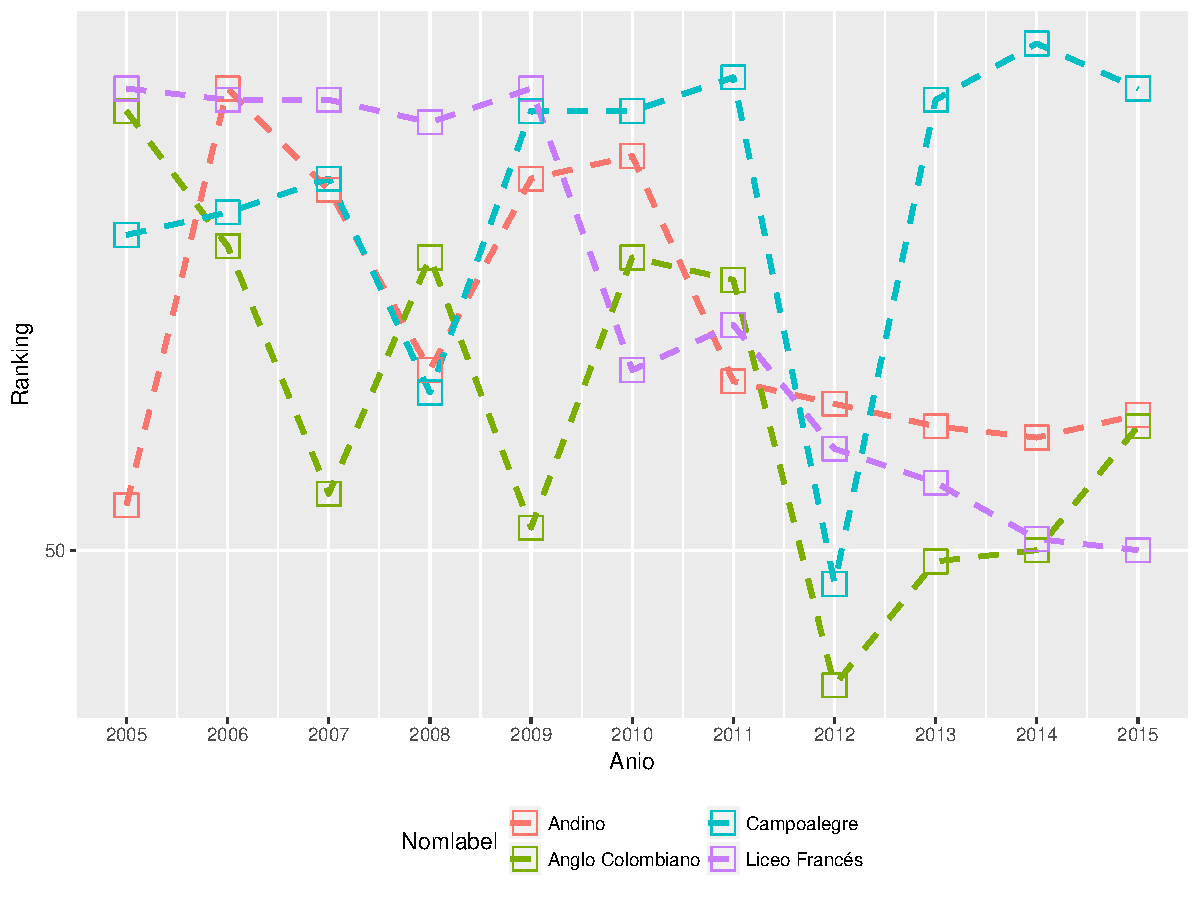
\includegraphics[width=.9\linewidth]{figure/rankings-1} \caption[El ranking se calcula promediando los resultados de cada colegio en cada materia de la prueba SABER 11]{El ranking se calcula promediando los resultados de cada colegio en cada materia de la prueba SABER 11. Fuente: ICFES}\label{fig:rankings}
\end{figure}


\end{knitrout}
\end{center}

\newpage
\begin{center}
{\bf\Huge{PUESTOS INDIVIDUALES EN SABER 11}}\\
\vspace{0.1cm}
 Puesto de los colegios a nivel nacional en el periodo 2005-2015
\end{center}
\vspace{2cm}
\begin{center}
\begin{knitrout}
\definecolor{shadecolor}{rgb}{0.969, 0.969, 0.969}\color{fgcolor}\begin{figure}[H]
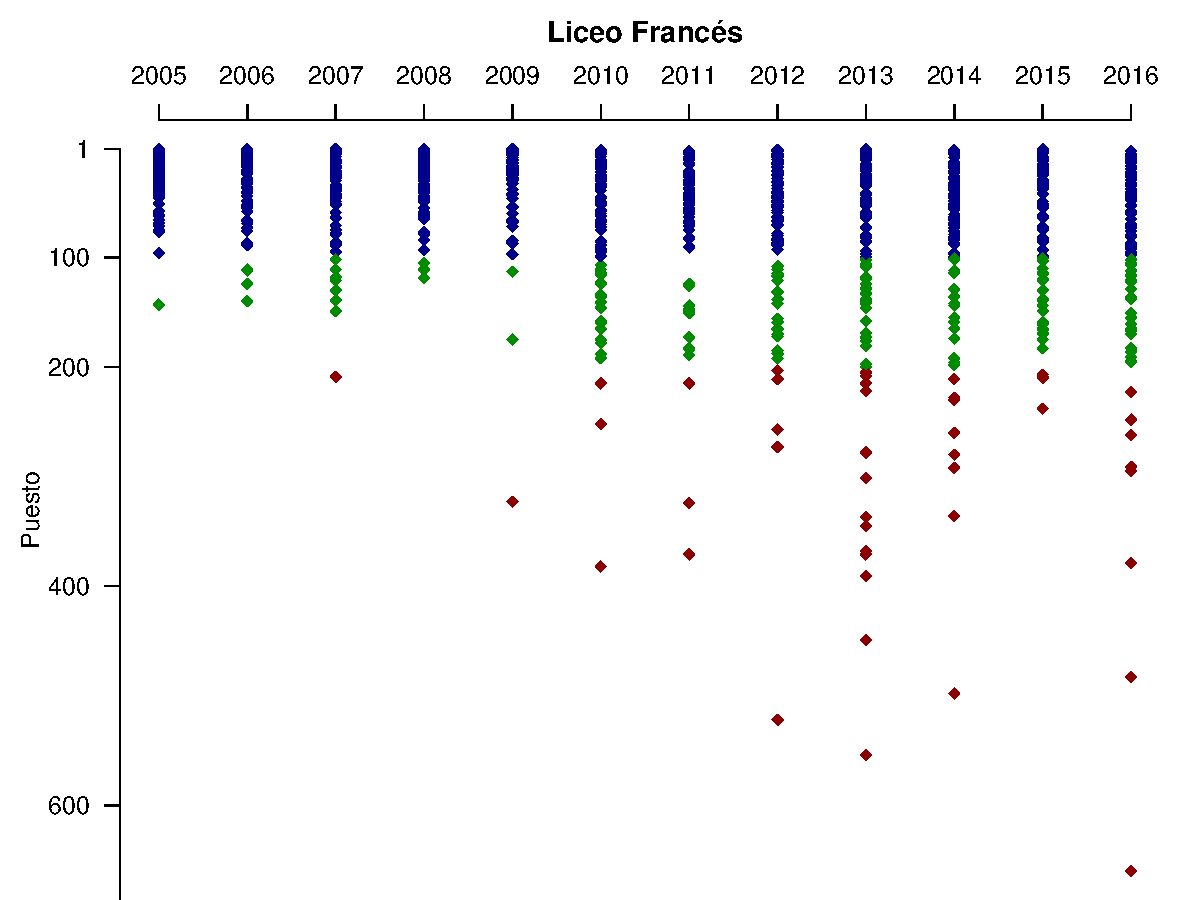
\includegraphics[width=.9\linewidth]{figure/pindiv-1} \caption[Cada estudiante obtiene un puesto entre el 1 y el 1000]{Cada estudiante obtiene un puesto entre el 1 y el 1000. Obtener el puesto 100 significa obtener un resultado superior al 90\% del país.}\label{fig:pindiv}
\end{figure}


\end{knitrout}
\end{center}

\newpage
\begin{center}
{\bf\Huge{UNIVERSIDADES}}\\
\vspace{0.1cm}
 Porcentaje de exalumnos de cada colegio graduados de las universidades del país en el periodo 2011-2015.
\end{center}
\vspace{2cm}
\begin{center}
\begin{knitrout}
\definecolor{shadecolor}{rgb}{0.969, 0.969, 0.969}\color{fgcolor}\begin{figure}[H]
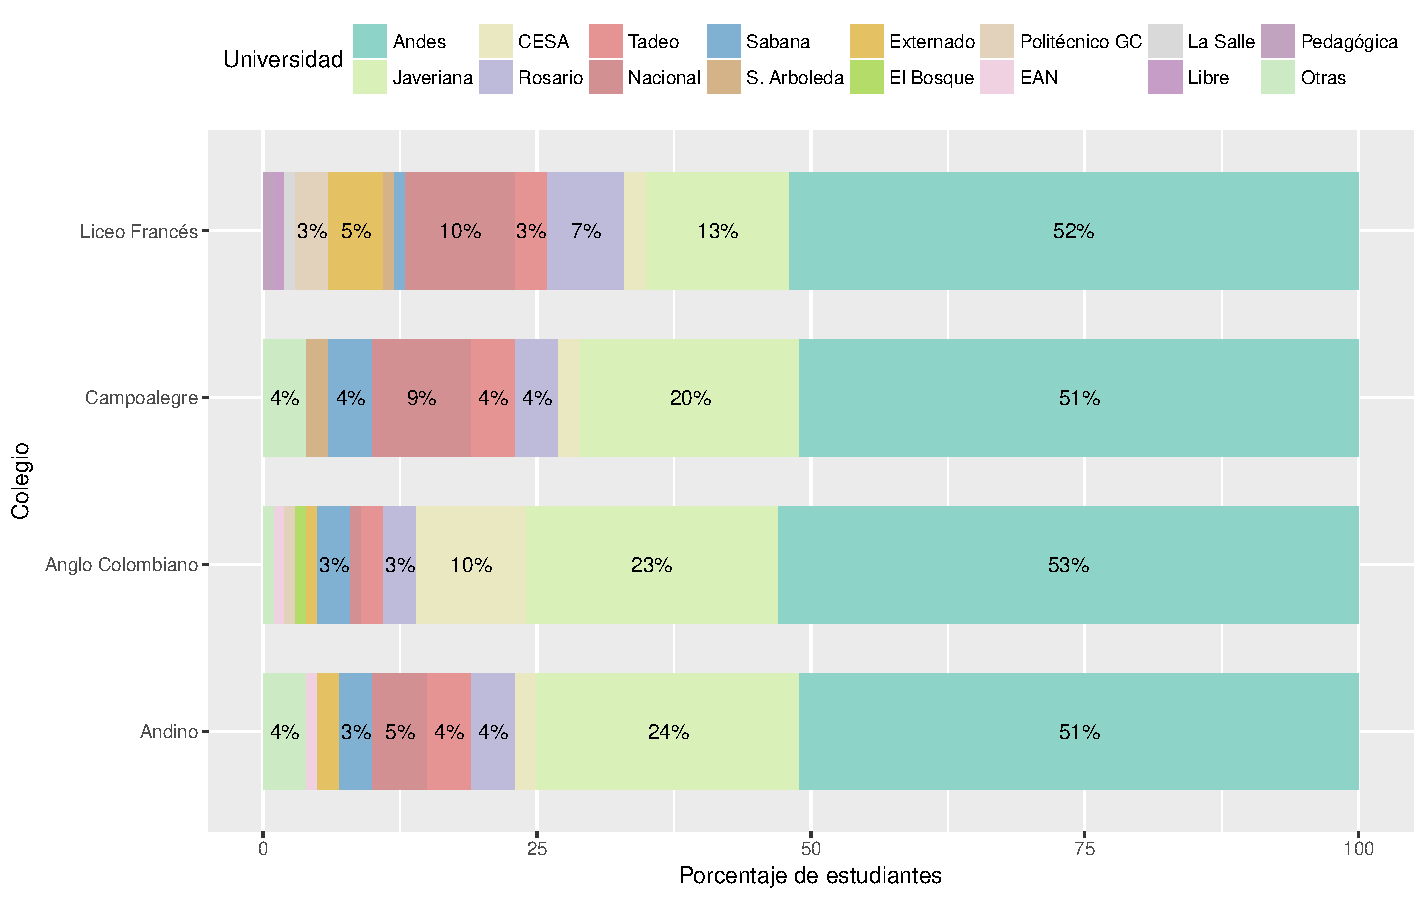
\includegraphics[width=.9\linewidth]{figure/graphuniv-1} \caption[ ]{ }\label{fig:graphuniv}
\end{figure}


\end{knitrout}
\end{center}

\newpage
\begin{center}
{\bf\Huge{CARRERAS}}\\
\vspace{0.1cm}
 Porcentaje de exalumnos de cada colegio graduados de las universidades del país en el periodo 2011-2015.
\end{center}
\vspace{2cm}
\begin{center}
\begin{knitrout}
\definecolor{shadecolor}{rgb}{0.969, 0.969, 0.969}\color{fgcolor}\begin{figure}[H]
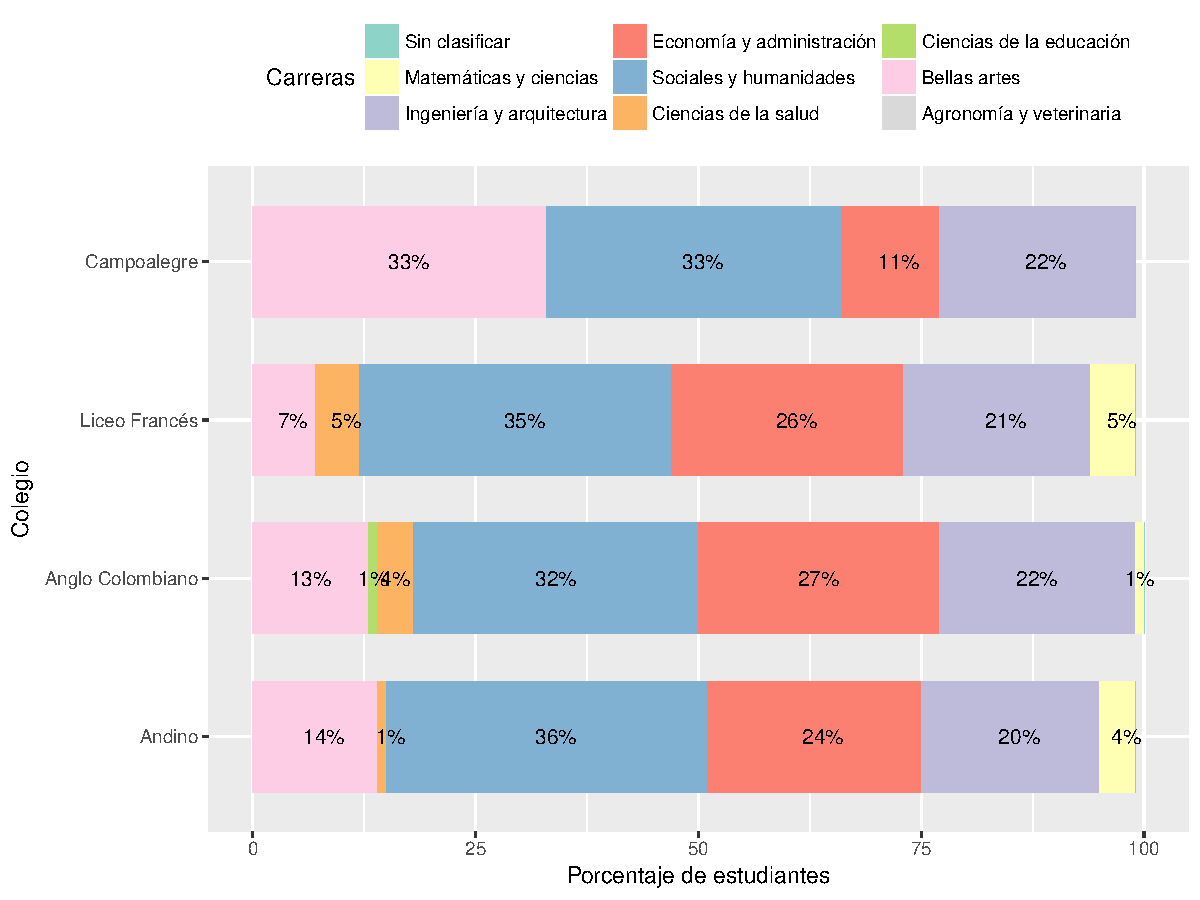
\includegraphics[width=.9\linewidth]{figure/graphcarr-1} \caption[ ]{ }\label{fig:graphcarr}
\end{figure}


\end{knitrout}
\end{center}




\newpage
\begin{center}
{\bf\Huge{COMPARACION DE COLEGIOS}}\\
\vspace{0.1cm}
 Según los criterios elegidos por la familia de Agustín Ramírez Carrizosa
\end{center}


\vspace{1cm}

% latex table generated in R 3.4.1 by xtable 1.8-2 package
% Tue Oct 10 13:28:41 2017
\begin{table}[ht]
\centering
\begin{tabular}{C{1in}C{1in}C{1in}C{1in}C{1in}}
  \hline
 & Andino & Anglo Colombiano & Liceo Francés & Campoalegre \\ 
  \hline
Prioridad Alemán & Segundo &  &  &  \\ 
  Rango infraestructura deportiva &  &  &  &  \\ 
  Grado inicio segundo idioma & Preescolar & Preescolar & Preescolar & Preescolar \\ 
  ¿Hay estudiantes necesida especial? &  &  &  & Asperger/OCD/ADD \\ 
  ¿Son incluídos? &  & si & si & si \\ 
  Rango aprox. tiempo a Chicó en carro & 41 & 44 &  3 & 80 \\ 
  Rango tecnología & Promedio & Superior & Promedio & Baja \\ 
   \hline
\end{tabular}
\end{table}


\vspace{0.5cm}

\begin{itemize}
\item Descripción
\item Descripción de la infraestructura deportiva, horarios
\item Descripción:intensidad
\item Descripción de las necesidades especiales, casos
\item ¿por qué sí?
\item Datos tomados en tales horas
\item Descripción de lad tecnologías
\end{itemize}
\newpage

%\ContraPortada
\ClearShipoutPicture

\includepdf{Backgrounds/contraportada.pdf}
\end{document}


%FIN DEL DOCUMENTO
%en el comment van ejemplos de usos de las opciones red, blue del eccooleinfauto.sty
\begin{comment}
\noindent
Let's begin with a simple working example here.


\section{Introduction}
In this document a new package is tested. This package allows special numbered
environments

\begin{example}
This text is inside a special environment, some boldface text is printed
at the beginning and a new indentation is set.
\end{example}

Also, there's a special command for \important{important!words} that will be
printed in a special \important{colour} depending on the parameter used in the
\important{package} importation statement. Because it's \important{important}.




\section{colegios}

The Monty Hall problem...
The Monty...


\end{comment}
